\subsection{Relatório Consolidado - Avaliação 1 Acessibilidade}

\flushleft \textbf{Data da avaliação:} 
06/06/2015

\textbf{Objetivo:}
Avaliar a acessibilidade da aplicação, ou seja, o quanto ela está adequada para pessoas portadoras de algum tipo
de necessidade especial.

\textbf{Método:}
Ferramenta ASES.

\textbf{Dados coletados:}
Para construção desse protótipo foram levadas em consideração as características contidas na Tabela \ref{tab:emag} e 
as considerações provenientes do \cite{emag}. Assim, este protótipo foi construído de forma a obter um resultado
satisfatório no quesito acessibilidade.

Os dados coletados na ferramenta ASES podem ser vistos na Figura \ref{fig:avaliacao_ases1}.

\begin{figure}[h!]
  \centering
    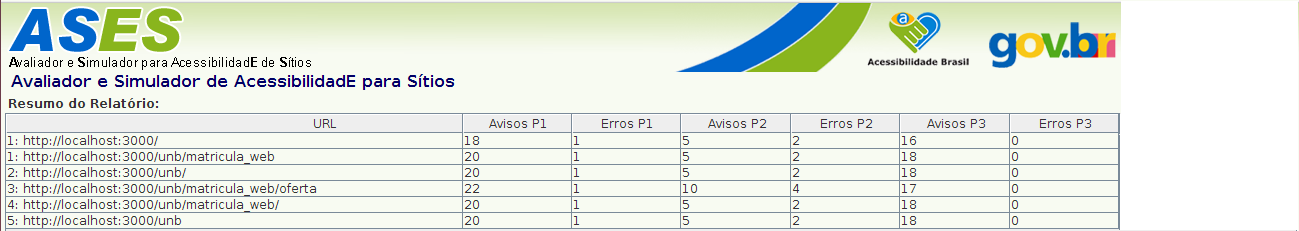
\includegraphics[keepaspectratio=true, scale=0.6]{figuras/avaliacao_ases1.png}
  \caption{Resultado da primeira avaliação da ferramenta ASES}
  \label{fig:avaliacao_ases1}
\end{figure}

Também foi avaliado o contraste de cor entre alguns objetos da tela. Os dados da avaliação contraste podem ser vistos nas Figuras \ref{fig:contraste1} e \ref{fig:contraste1b}.

Na Figura \ref{fig:contraste1}a está representado o contraste entre o fundo do menu e os links e na \ref{fig:contraste1}b entre a cor do botão e o nome de pesquisa.
\begin{figure}[h!]
  \centering
  \subfloat[a]{
    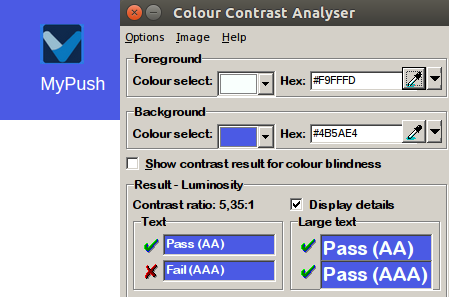
\includegraphics[keepaspectratio=true, scale=0.6]{figuras/contraste1.png}
   }
   \subfloat[b]{
      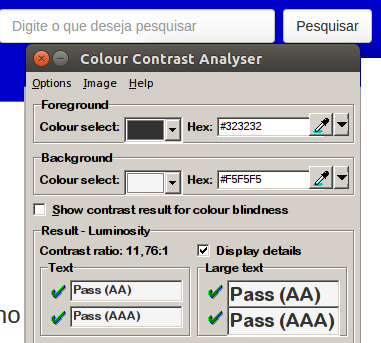
\includegraphics[keepaspectratio=true, scale=0.6]{figuras/contraste_pesquisa.png}
   }
    \caption{Resultado da avaliação de contraste}
    \label{fig:contraste1}
\end{figure}

Na Figura \ref{fig:contraste1b}a está representado o contraste entre o fundo da página e o texto escrito e na \ref{fig:contraste1b}b entre o fundo da página e a seta.
\begin{figure}[h!]
  \centering
  \subfloat[a]{
    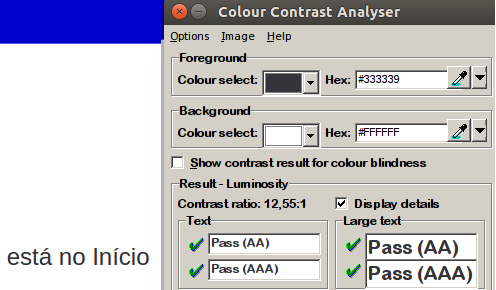
\includegraphics[keepaspectratio=true, scale=0.5]{figuras/contraste_palavra.png}
   }
   \subfloat[b]{
      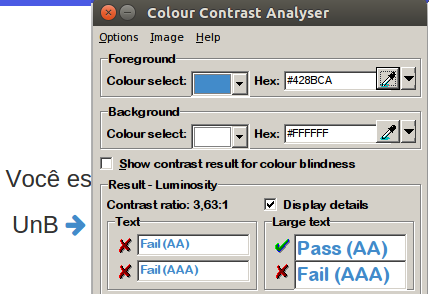
\includegraphics[keepaspectratio=true, scale=0.5]{figuras/contraste_seta1.png}
    }
    \caption{Resultado da avaliação de contraste}
    \label{fig:contraste1b}
\end{figure}

\textbf{Planejamento para a próxima versão do protótipo:}
A partir dos dados coletados serão feitos os ajustes recomendados pela ferramenta ASES e serão procuradas cores que passem em todas
as categorias da avaliação de contraste.

\vfill
\pagebreak


\subsection{Relatório Consolidado - Avaliação 2 Acessibilidade}

\flushleft \textbf{Data da avaliação:} 
20/06/2015

\textbf{Objetivo:}
Avaliar a acessibilidade da aplicação, ou seja, o quanto ela está adequada para pessoas portadoras de algum tipo
de necessidade especial.

\textbf{Método:}
Ferramenta ASES e \textit{Colour Contrast Analyser}.

\textbf{Dados coletados:}
Após as melhorias feitas com base na primeira avaliação, os dados coletados na ferramenta ASES podem ser vistos na Figura \ref{fig:avaliacao_ases}.

\begin{figure}[h!]
  \flushleft
    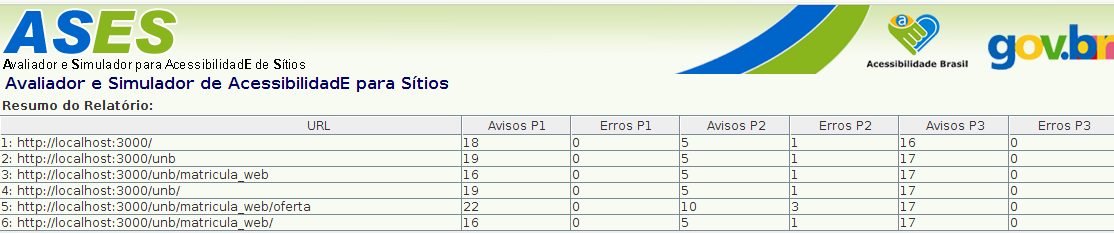
\includegraphics[keepaspectratio=true, scale=0.6]{figuras/avaliacao_ases.png}
  \caption{Resultado da segunda avaliação da ferramenta ASES}
  \label{fig:avaliacao_ases}
\end{figure}

Com essa avaliação é notório que a aplicação tem poucos erros em relação à acessibilidade e possui alguns avisos.
A partir desses avisos foi possível ajustar o código de modo a deixar a aplicação mais acessível, contudo a ferramenta não
identificou esses ajustes. Assim, o erro que persistiu após a avaliação foi ajustado no código, mas não foi reconhecido pela ferramenta.

Também foi avaliado o contraste de cor entre os objetos que mudaram de cor desde a última avaliação. As avaliações podem ser vistas nas Figuras 
\ref{fig:contraste2}. Na Figura \ref{fig:contraste2}a está representado o contraste entre o fundo do menu e os links e na \ref{fig:contraste2}b entre o fundo da página e a seta.

\begin{figure}[h!]
  \centering
  \subfloat[a]{
    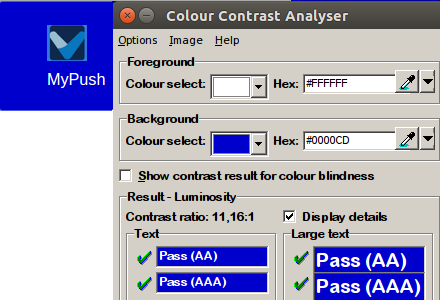
\includegraphics[keepaspectratio=true, scale=0.5]{figuras/contraste2.png}
   }
   \subfloat[b]{
      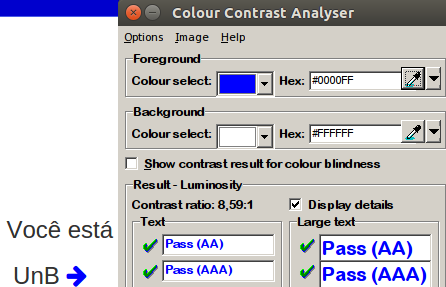
\includegraphics[keepaspectratio=true, scale=0.5]{figuras/contraste_seta2.png}
   }
    \caption{Resultado da avaliação de contraste}
    \label{fig:contraste2}
\end{figure}



\textbf{Planejamento para a próxima versão do protótipo:}
Como os ajustes foram feitos mas não identificados pela ferramenta, o protótipo foi considerado estável para o seu fim.

\vfill
\pagebreak




